\chapter{Results and discussion}
\label{chap:results}

Our approach of integrating Embree into ART, as outlined in the previous chapter, was tested on a variety of scene files. This chapter provides an overview and analysis of the performance of our implementation. It is divided into three sections. Subsection \ref{sec:results_csg} discusses the execution time of ART when rendering scenes containing constructive solid geometries. A comparison is drawn between our two approaches for realizing CSG operations with Embree, the initialization of an entire CSG as a user-defined geometry and the traversal through the original scene graph or a dedicated KD tree. We will exclude the provision of results concerning the rendering of CSG through the collection of intersection points and their subsequent evaluation, outlined in Subsection \ref{subsec:apprach1}. This exclusion is due to the significantly decreased rendering performance resulting from this approach, and thus, making it impractical.

Furthermore, we decided to test our implementation on virtual scenes, using mesh geometry, to analyze and compare the performance of rendering non-user-defined and user-defined geometries. 

Section \ref{sec:result_normal} provides the results on various scenes rendered by an hybrid implementation combining the approaches outlined in Subsections \ref{subsec:apprach2} and \ref{subsec:apprach3}. 

In Section \ref{sec:result_meshes}, we test and evaluate our implementation on scene exclusively composed of triangles with varying amount of geometry.

The following experiments were conducted on an Asus N551JX laptop with a quad-core Intel Core i7–4720HQ processor clocked at 2.6 GHz and 8 GB of RAM. The images shown in this chapter were rendered in ART with Embree support at a resolution of 700x700, a path length of 20, and 128 samples per pixel. The internal calculations regarding the image synthesis of these scenes were performed via multi-threading with eight threads.

\section{Evaluation of our integration for scenes containing CSG}
\label{sec:results_csg}

We tested the functionality of our implementation concerning CSG rendering with Embree on six scenes, which were made publicly available by the developers of ART \footnote{Most of the scenes shown in this chapter can be found in the \texttt{Gallery} folder of the ART repository, which is submitted together with this thesis as an electronic attachment. Scenes or 3D models that are not taken from this folder will be cited.}. All the scenes mentioned in this section contain an infinite sphere, serving as a skydome to light the scene. 
\\

\noindent For this evaluation, our implementation was tested on the following scenes:
\begin{itemize}
	\setlength\itemsep{0.05em}
	
	\item The scene shown in Figure \ref{fig:csg_shell} consists of a single CSG, a procedurally modeled shell, and multiple cubes aligned to form a checkerboard pattern. The CSG, namely the shell, is composed of a total amount of 2,144 sphere primitives. The shell is modeled by arranging the spheres in spiral form and decreasing order according to their sizes. The largest sphere at the beginning of this sequence of spheres is "subtracted" by the \texttt{SUB} operator from the rest of the spheres. Then, the next largest sphere is "unified" by the \texttt{OR} operator with its preceding sphere in the sequence. This procedure is repeated for the remaining spheres in the sequence.
	
	\item  Figure \ref{fig:csg_orennayar} shows the rendered image of a scene composed of a cylinder serving as the ground on which three so-called \emph{grooved spheres} are placed. The grooves on the sphere result from applying a \texttt{SUB} operator to a group of six tori and the sphere in question.
	The purpose of this scene is to showcase ART's implementation of the Oren–Nayar reflectance model \cite{oren1994generalization} with different roughness grades.
	
	\item We have already encountered the Villa Rotonda scene in Subsection \ref{subsec:apprach1}. As mentioned there, the model of the Villa Rotonda is composed of two CSG with a total number of 1,255 primitives.
		
	\item The scene displayed in Figure \ref{fig:csg_torrancesparrow} is composed of twelve grooved spheres that are placed on three deformed cubes with different heights that together form a staircase. Furthermore, a cylinder serves as the ground. The initial purpose of this particular scene was the demonstration of the implementation of the Torrance–Sparrow reflectance model \cite{torrance1967theory} with varying roughness grades.
	
	\item Figure \ref{fig:csg_plane} shows a rendered image of a scene composed of a cylinder acting as the ground, and a biplane, composed of multiple CSG. The total number of topmost CSG nodes in the scene graph assembled by ART for this particular scene amounts to 28. The total number of geometric primitives of the 28 CSG is 336.
	
	\item Lastly, the rendered scene shown in Figure \ref{fig:csg_locomotive} shows a model of an Austrian steam locomotive. The single model is composed of multiple CSG, a total amount of 354 topmost CSG nodes are present in the scene graph associated with this scene The amount of geometric primitives present in the scene is 3,594.
	
	
\end{itemize}

\begin{figure}
	\centering
	\subfloat[Shell]{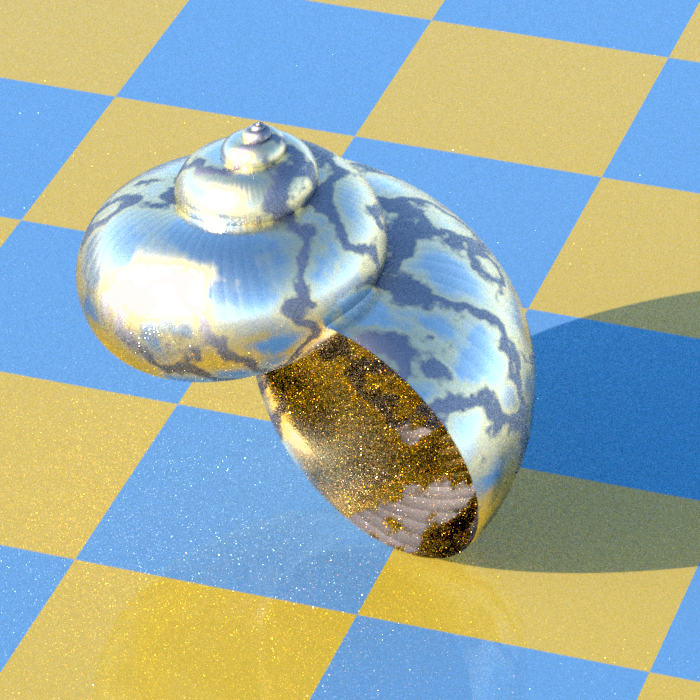
\includegraphics[width=.3\textwidth]{img/4 results/csg/snailEmbree.png}\label{fig:csg_shell}}
	\hfill
	\subfloat[Oren-Nayar Sphreres]{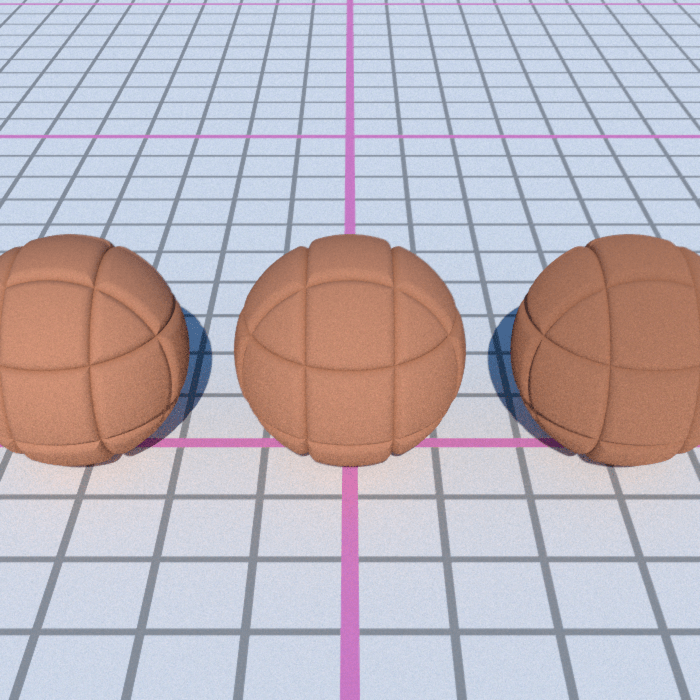
\includegraphics[width=.3\textwidth]{img/4 results/csg/orennayarEmbree.png}\label{fig:csg_orennayar}}
	\hfill
	\subfloat[Villa Rotonda]{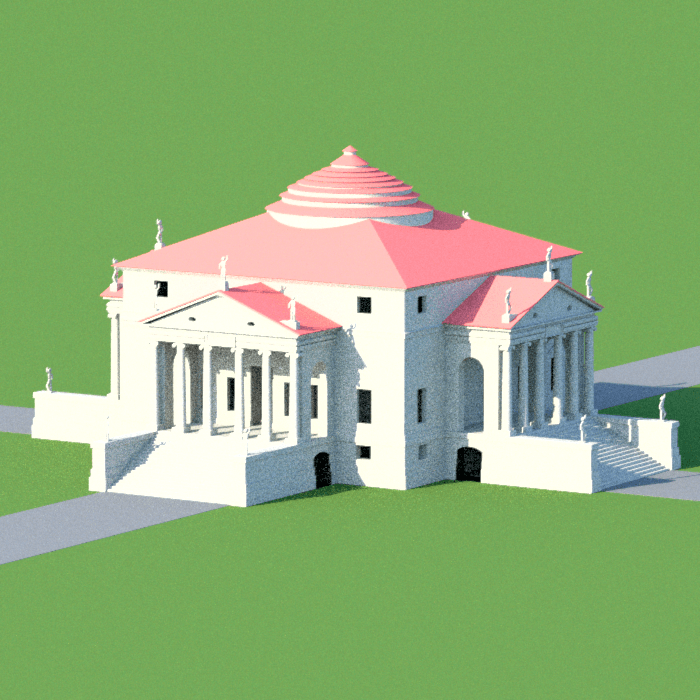
\includegraphics[width=.3\textwidth]{img/4 results/csg/rotondaEmbree.png}\label{fig:csg_rotonda}}
	\\
	\subfloat[Torrance-Sparrow Spheres]{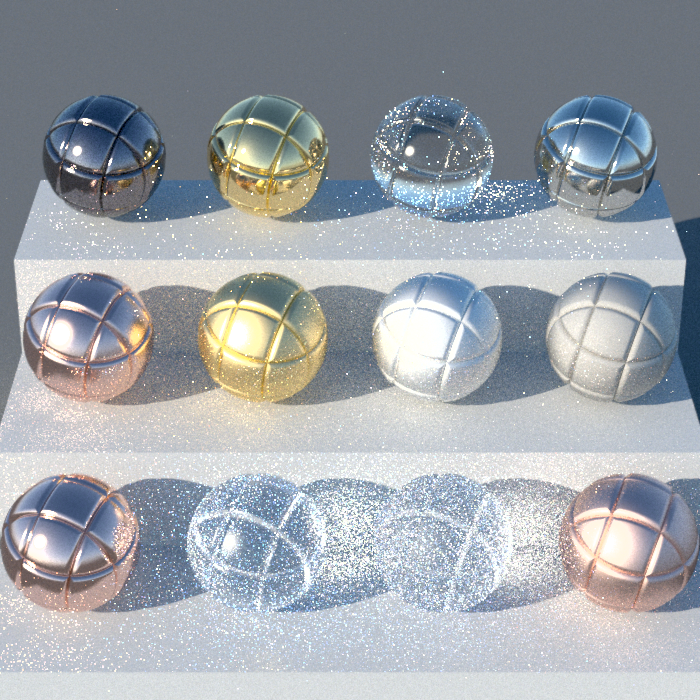
\includegraphics[width=.3\textwidth]{img/4 results/csg/torrancesparrowEmbree.png}\label{fig:csg_torrancesparrow}}
	\hfill
	\subfloat[Parked Biplane]{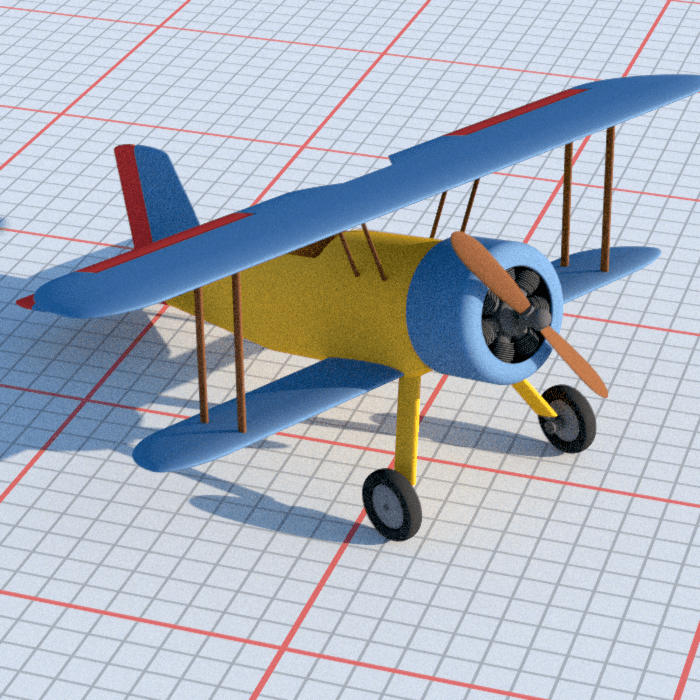
\includegraphics[width=.3\textwidth]{img/4 results/csg/planeEmbree.png}\label{fig:csg_plane}}
	\hfill
	\subfloat[Locomotive]{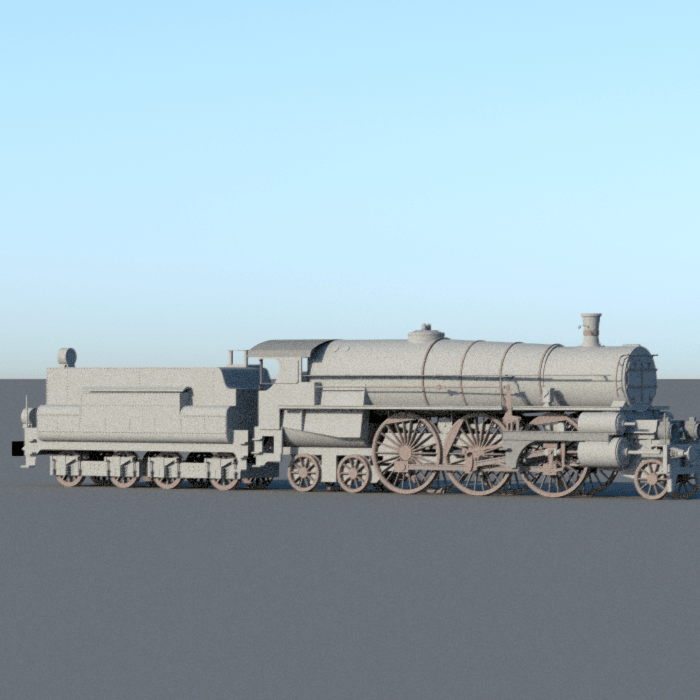
\includegraphics[width=.3\textwidth]{img/4 results/csg/locomotiveEmbree.png}\label{fig:csg_locomotive}}
	
	\caption{Scenes containing CSG, rendered with our implementation. The image of the Villa Rotonda shown in Figure \ref{fig:csg_rotonda} was rendered by traversing KD trees associated with the CSG in this scene. Unfortunately, the issue described in Subsection \ref{subsec:apprach2} remains when rendering the scene by traversing the original scene graph.}
	\label{fig:csg_figures}
\end{figure}

\begin{table}[h]
	\centering
	{\footnotesize\sf
		\begin{tabular}{lrrrrrr}
			\toprule
			Scene & \thead{\texttt{\#}Topmost \\ CSG \\ nodes} & Native ART & \thead{Org scene \\ graph} &  KD tree & \thead{Org scene \\ graph \\ speedup} & \thead{KD tree \\ speedup} \\ 
			\midrule
			Figure \ref{fig:csg_shell} & 1 & 2,611.75 sec & 2,437.81 sec & 4,151.01 sec & \textbf{6.66 \%} & \textbf{\textcolor{red}{-58.94 \%}}  \\
			Figure \ref{fig:csg_orennayar} & 3 & 791.71 sec & 522.97 sec & 528.77 sec & \textbf{33.94 \%} & \textbf{33.21 \%} \\
			Figure \ref{fig:csg_rotonda} & 2 & 738.25 sec & 629.03 sec &  765.44 sec & \textbf{14.79 \%}  & \textbf{\textcolor{red}{-3.68 \%}}  \\
			\addlinespace % a nice non-intrusive separator of data groups (or final table sums)
			Figure \ref{fig:csg_torrancesparrow} & 12 & 910.56 sec & 896.97 sec & 902.61 sec & \textbf{1.49 \%}  & \textbf{0.87 \%} \\
			Figure \ref{fig:csg_plane} & 28 & 522.58 sec & 498.25 sec & 546.79 sec & \textbf{4.66 \%} & \textbf{\textcolor{red}{-4.63} \%} \\
			Figure \ref{fig:csg_locomotive} & 354 & 312.94 sec & 272.08 sec & 280.83 sec & \textbf{13.06 \%}  & \textbf{10.26 \%} \\
			\bottomrule
	\end{tabular}}
	\caption{Comparison between the performances of Native ART and ART with Embree support. The performance of both methods of traversing the original scene graph and traversing the dedicated KD tree is compared to the performance of Native ART.}
	\label{tab:csg}
\end{table}

The results we obtained from these tests show that rendering CSG geometry by traversing the original scene graph is competitive with Native ART. For the scene shown in Figure \ref{fig:csg_torrancesparrow}, the speedup resulting from the support of Embree is only marginal. However, the increased acceleration shown in the table for the scene shown in Figure \ref{fig:csg_orennayar} is indeed noteworthy. We want to emphasize that the overall acceleration shown in the table is not just thanks to Embree but also the fast traversal of the subgraphs of ART's interior scene graph representing the CSG in the scene.

The results we obtained by traversing KD trees that are associated with CSG are highly scene dependent. For the scenes shown in Figures \ref{fig:csg_orennayar}, \ref{fig:csg_torrancesparrow} and \ref{fig:csg_locomotive}, this approach is comparable to the approach of traversing the original scene graph. However, for scenes shown in Figures \ref{fig:csg_shell}, \ref{fig:csg_rotonda} and \ref{fig:csg_plane} the rendering time increased compared to Native ART. The decrease seen in the table for Figures \ref{fig:csg_rotonda} and \ref{fig:csg_plane} can arguably be regarded as competitive with Native ART. Nevertheless, the decrease of performance regarding the rendering of the scene shown in Figure \ref{fig:csg_shell} is significant. These three scenes have in common that they contain CSG being constructed from a large number of geometric primitives. Therefore, these CSG are associated with complex KD trees whose traversal impacts the performance. In contrast, the locomotive model shown in Figure \ref{fig:csg_locomotive}, which is constructed by a large number of primitives, too, is modeled by the assembly of multiple CSG instead of one single large one. This explains why we did not experience a decrease in performance regarding this scene.

We conclude that our approach of traversing KD trees associated with CSG does work well with CSG composed of a manageable amount of geometric primitives but does not work well with more complex CSG.

\subsubsection{Special case: Rendering CSG composed of triangle meshes}

\begin{figure}[h]
	\centering
	\subfloat[Scene rendered with native ART by traversing the internal KD tree.]{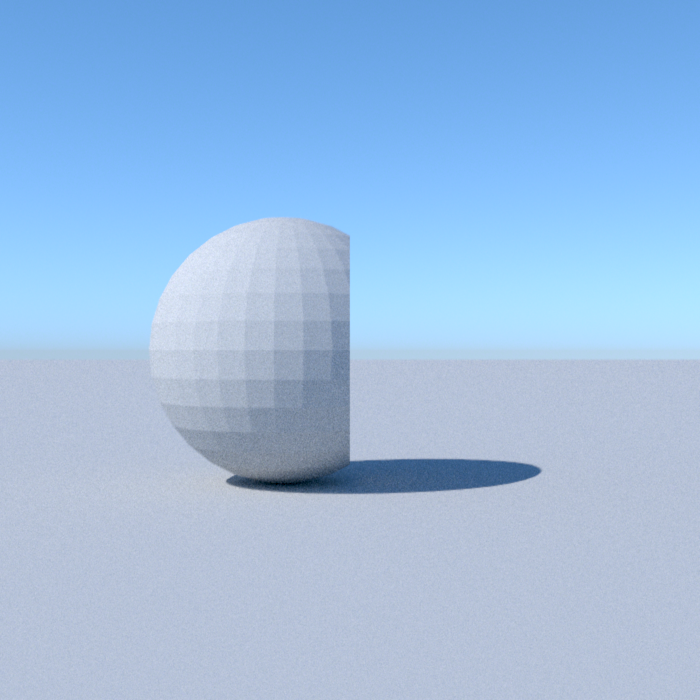
\includegraphics[width=.4\textwidth]{img/3 approach/spheresEmbree.png}\label{fig:csg_mesh_spheres}}
	\hfil
	\subfloat[Artifact in the scene rendered with the approach outlined in this section.]{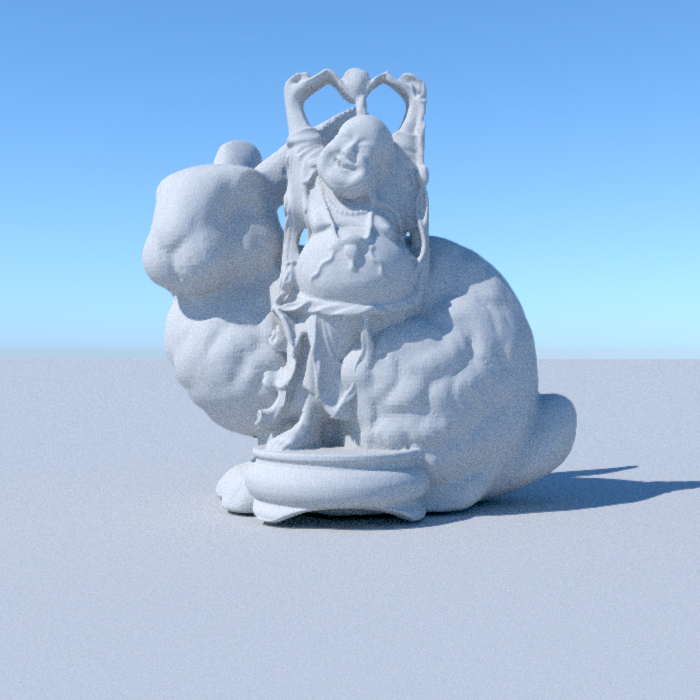
\includegraphics[width=.4\textwidth]{img/4 results/csg/meshCSGEmbree.png}\label{fig:csg_mesh_bunny_buddha}}
	\caption{CSG composed of triangle meshes. The figures show a scene with two spheres described as triangle meshes. The right sphere is "subtracted" from the left sphere via the Boolean set operation \texttt{OR}. The scene can be regarded as the counterpart of the scene shown in Figure \ref{fig:csg_sub} for triangle mesh primitives.}
	\label{fig:csg_mesh_results}
\end{figure}

\begin{table}[h]
	\centering
	{\footnotesize\sf
		\begin{tabular}{lrrrrr}
			\toprule
			Scene  & \thead{Native ART \\ Preparation} & \thead{Native ART \\ Ray \\ Tracing} & \thead{Embree \\ Preparation} & \thead{Embree \\ Ray Tracing} & \thead{Ray Tracing \\ Speedup} \\ 
			\midrule
			Figure \ref{fig:csg_mesh_spheres} & 0.09 sec & 237.25 sec & 0.09 sec & 284.86 sec & \textbf{\textcolor{red}{-20.07 \%}} \\
			Figure \ref{fig:csg_mesh_bunny_buddha} & 4.58 sec & 376.20 sec & 61.82 sec & 709.77 sec  & \textbf{\textcolor{red}{-88.67 \%}} \\
			\bottomrule
	\end{tabular}}
	\caption{Comparison between the performances of Native ART and ART with Embree support. The time needed for preparing the ray tracing process by constructing the internal acceleration data structures and the time needed for the ray tracing process itself.}
	\label{tab:csg_mesh}
\end{table}

For testing our implementation on scenes that contain CSG, which are composed of triangle meshes, we modeled two scenes. Figure \ref{fig:csg_mesh_spheres} shows the rendered image of a scene, composed of a quadrangle and two spheres that are described by triangle meshes. The right sphere is "subtracted" from the left sphere by applying the difference set operation. Figure \ref{fig:csg_mesh_bunny_buddha} shows the rendered image of a scene that contains again of a quadrangle, and two triangle meshes provided by the Stanford 3D Scanning Repository \cite{plyRepo}, namely the Stanford Bunny, composed of 69,451 triangles and the Happy Buddha, composed of 1,087,716 triangles. The results are shown in Table \ref{tab:csg_mesh}.
As described in Subsection \ref{subsec:apprach2}, ray tracing these types of CSG is not possible with our approach of traversing the original scene graph. Therefore, the results shown refer to the approach of traversing individual KD trees associated with the CSG.

The results in the table indicate a significant decrease in ray tracing performance when rendering CSG composed from triangle meshes. This drop-off can be explained the following way: Embree was originally developed for rendering scenes containing complex geometry, being described by a high number of primitives. Therefore, it does not perform well with scenes containing a small number of geometries. In our scenes, only two geometries are present, a plane and the entire CSG. Furthermore, the combining of Embree's BVHs and ART's internal KD trees for such simple scenes does not accelerate the intersection calculation process. It, in fact, complicates it.

We do not recommend using our approach to render CSG composed of triangle meshes at the current stage. 


\section{Hybrid implementation and evaluation}
\label{sec:result_normal}

After examining the results of our tests concerning the rendering of CSG described in the previous section, we decided to abandon our approach of calculating the intersection points by traversing KD trees associated with the CSG in the scene. For now, we accept the drawback concerning the Villa Rotonda scene missing its roof, as outlined in Subsection \ref{subsec:apprach2}, as a known issue.

However, we cannot completely abandon the approach of building and traversing individual KD trees for CSG since scenes with CSG that are composed of at least one triangle mesh strictly depend on these. Therefore, in our final implementation, we use a hybrid technique merging our approaches described in Subsection \ref{subsec:apprach2} and Subsection \ref{subsec:apprach3}. During the preparation of the scene for ray tracing in ART, the scene graph is assembled. If, during the assembly, a topmost CSG node is encountered, we check if at least one of the leaves of its subtree is associated with a triangle mesh. If this is the case, a flag associated with the CSG in question is activated. Whenever such a flag is activated for a CSG, the internal KD tree for the triangle mesh primitive is built, and an individual KD tree is built for the CSG.
When a ray intersects this particular CSG during the ray tracing procedure, the intersections will be calculated by the traversal of the associated KD tree.

The intersection calculations between rays and CSG that are not constructed of at least one triangle mesh are calculated by traversal of the scene subgraph rooted at the topmost CSG node corresponding to the particular CSG.

This section provides the results of tests conducted with this final implementation.
\\

\noindent In the following, we provide an overview of the scenes used for testing the overall performance of ART with Embree support:
\begin{itemize}
	\setlength\itemsep{0.05em}
	
	\item The scene shown in Figure \ref{fig:chart} contains a model of the Macbeth ColorChecker, a color calibration tool. This model comprises one larger deformed cube serving as the frame and 24 cubes depicting the colored samples. The chart is placed on a cylinder.
	
	\item Figure \ref{fig:gandalf} shows a typical Cornell Box scene with two additional image textures applied to the rear of the box and two a quadrangle on the right. The scene is composed of a total number of 20 non-user-defined geometries.
	
	\item The scene shown in Figure \ref{fig:glow} was created as part of the development of a model for describing the emission from glowing solid objects, described in  \cite{wilkie2011physically}. It consists of twelve spheres and a cylinder on which the spheres are placed.
	
	\item Figure \ref{fig:skydome} shows an image of a scene that was originally published in \cite{wilkie2013predicting}. The scene consists of CSG, user-defined geometries, and a triangle mesh. We will refer to this scene as \emph{Exoplanet scene} since it was used to showcase illumination on earth-like exoplanets.
	
	
\end{itemize}


\begin{figure}
	\centering
	\subfloat[Macbeth ColorChecker]{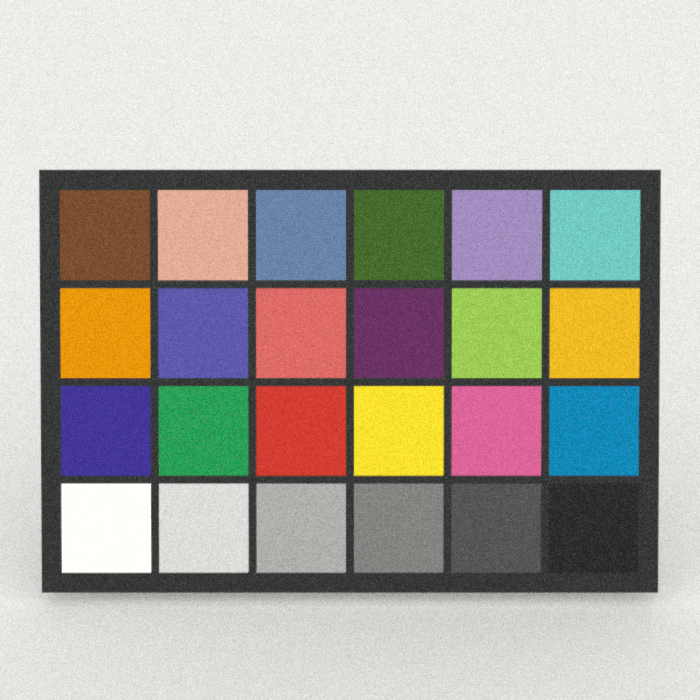
\includegraphics[width=.3\textwidth]{img/4 results/normal/chartEmbree.png}\label{fig:chart}}
	\hfill
	\subfloat[Cornell Box with texture mapping]{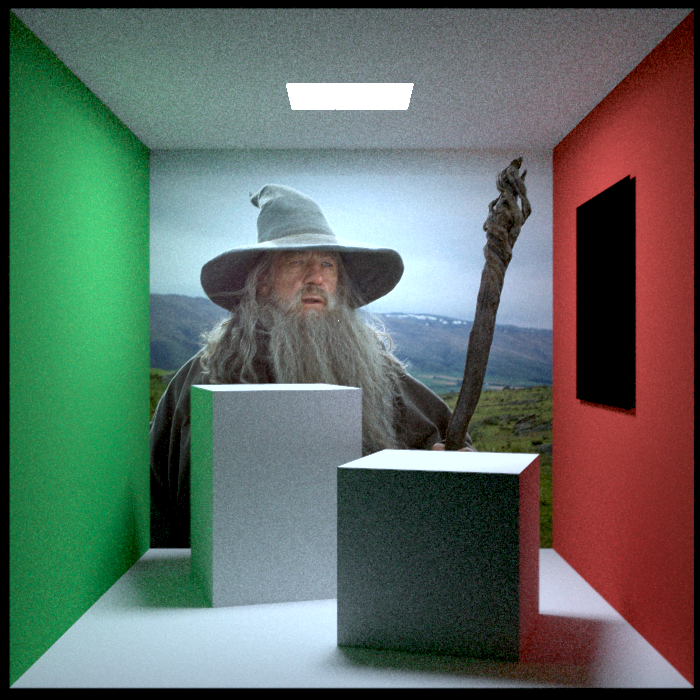
\includegraphics[width=.3\textwidth]{img/4 results/normal/imagemapEmbree.png}\label{fig:gandalf}}
	\hfill
	\subfloat[Glowing spheres]{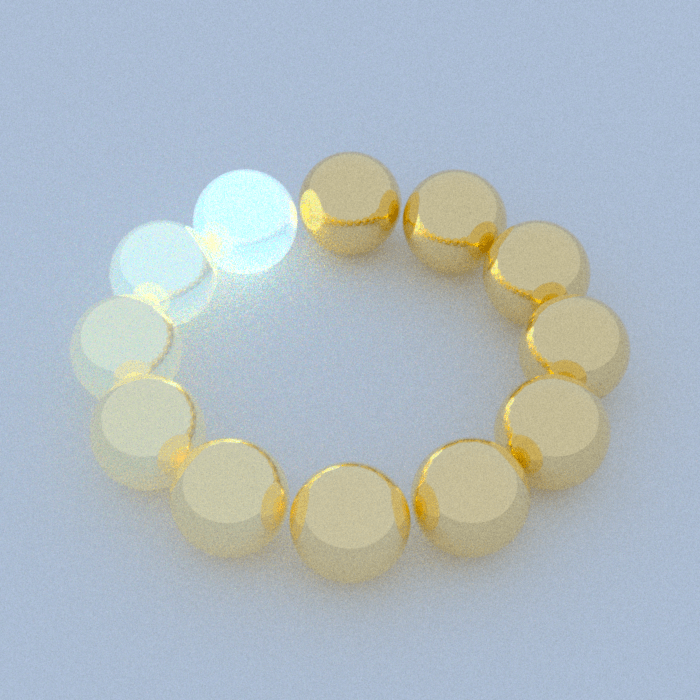
\includegraphics[width=.3\textwidth]{img/4 results/normal/glowEmbree.png}\label{fig:glow}}
	\\
	\subfloat[Exoplanet scene]{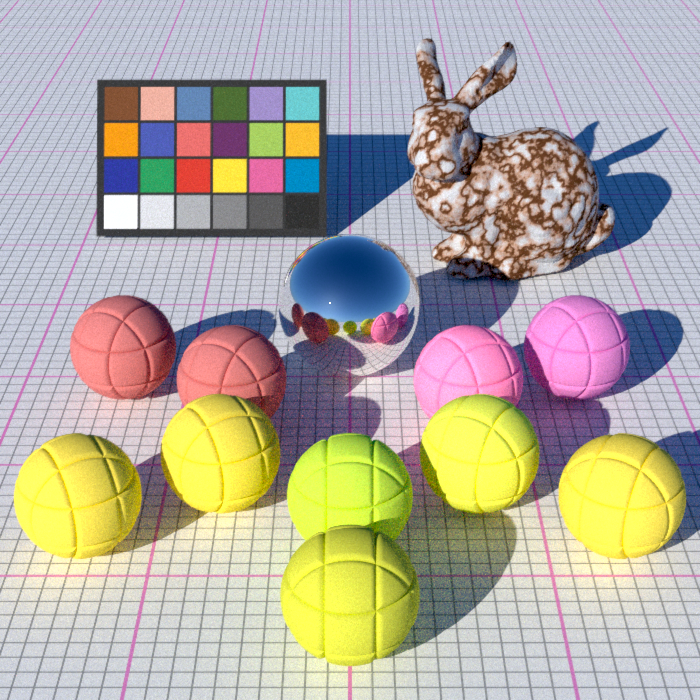
\includegraphics[width=.7\textwidth]{img/4 results/normal/skydomeEmbreeFinal.png}\label{fig:skydome}}

	\caption{Scenes containing various types of shapes: CSG, user-defined geometry, and non-user-defined geometry.}
	\label{fig:scenes}
\end{figure}


\begin{table}
	\centering
	{\footnotesize\sf
		\begin{tabular}{lrrrr}
			\toprule
			Scene & \Verb!#!Geometries & Native ART & Embree & Speedup \\ 
			\midrule
			Figure \ref{fig:chart} & 26 & 382.70 sec & 361.80 sec & \textbf{5.46 \%} \\
			Figure \ref{fig:gandalf} & 20 & 387.72 sec & 227.74 sec & \textbf{41.26 \%} \\
			Figure \ref{fig:glow} & 13 & 397.46 sec & 389.72 sec & \textbf{1.95 \%}  \\
			Figure \ref{fig:skydome} & 38 & 674.91 sec & 634.52 sec & \textbf{5.98 \%} \\
			\bottomrule
	\end{tabular}}
	\caption{Comparison between Native ART and our hybrid implementation on scenes that contain various types of geometries. In the table, triangle meshes and CSG are considered one geometry.}
	\label{tab:scenes}
\end{table}



\begin{figure}
	\centering
	\subfloat[Rendered image of the Cornell Box scene with the individual quadrangles being initialized with Embree's proprietary primitive types.]{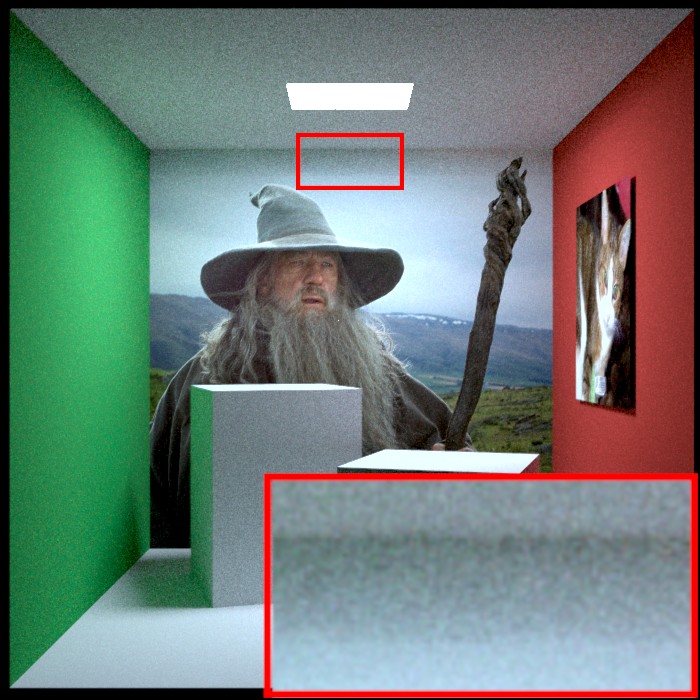
\includegraphics[width=.45\textwidth]{img/4 results/normal/imagemapEmbreeDetail.png}\label{fig:gandalf_embree}}
	\hfill
	\subfloat[Difference image between the image shown in Figure \ref{fig:gandalf_embree} and the corresponding image rendered by Native ART.]{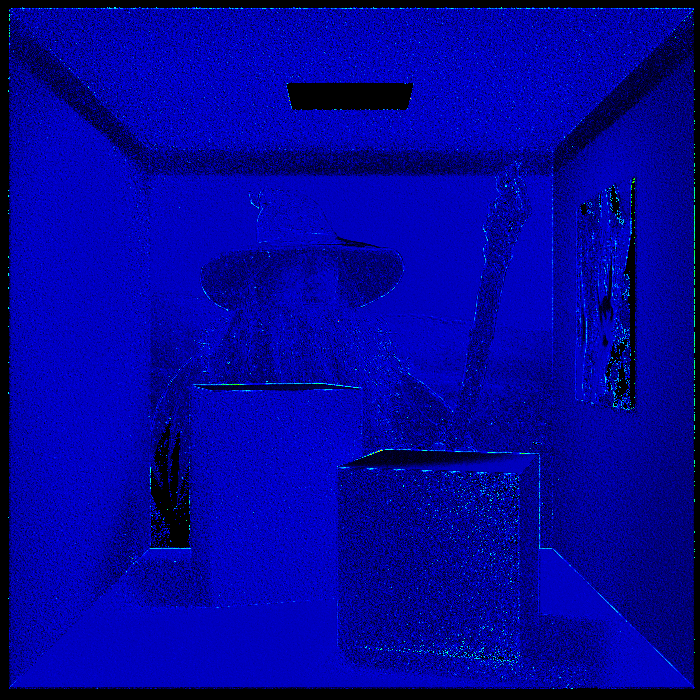
\includegraphics[width=.45\textwidth]{img/4 results/normal/differenceEmbreeNormal.png}\label{fig:difference_embree}}
	\\
	\subfloat[Rendered image of the Cornell Box scene with the individual quadrangles being initialized as user-defined geometries.]{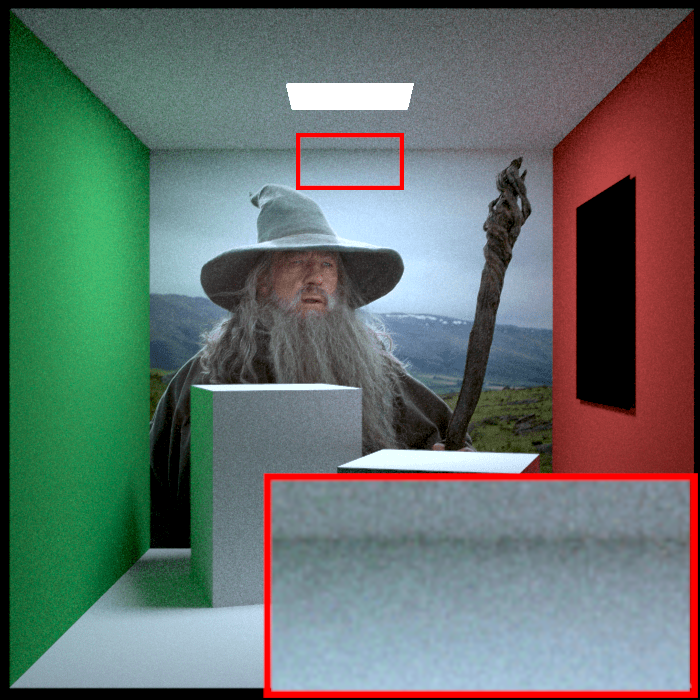
\includegraphics[width=.45\textwidth]{img/4 results/normal/imagemapEmbreeUserDetail.png}\label{fig:gandalf_embree_user}}
	\hfill
	\subfloat[Difference image between the image shown in Figure \ref{fig:gandalf_embree_user} and the corresponding image rendered by Native ART.]{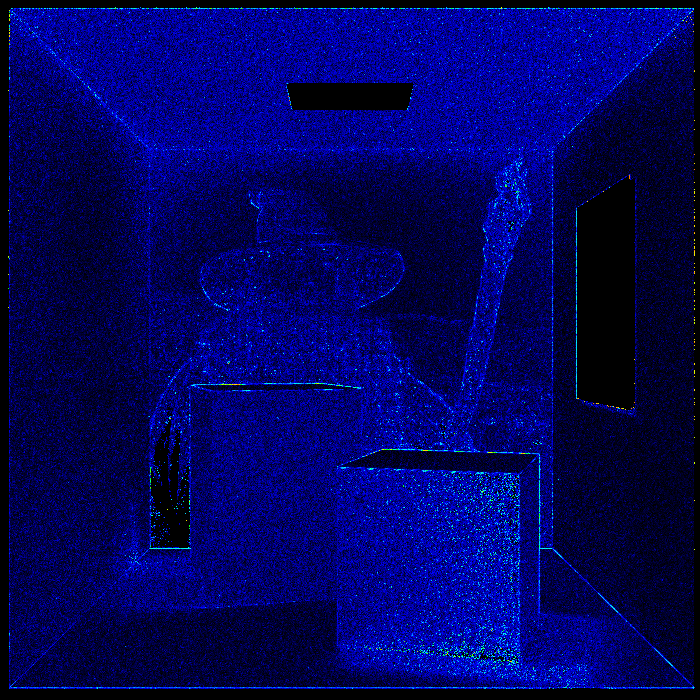
\includegraphics[width=.45\textwidth]{img/4 results/normal/differenceUserNormal.png}\label{fig:difference_embree_user}}
		
	\caption{Images of the Cornell Box scene rendered with different approaches.}
	\label{fig:res_gandalf_issue}
\end{figure}

The results shown in Table \ref{tab:scenes} are similar to those presented in Section \ref{sec:results_csg}. The result obtained by rendering the scene shown in Figure \ref{fig:gandalf} stands out from the remaining results. The performance speedup is due to this scene being modeled entirely with non-user-defined geometries, which are initialized with Embree's proprietary primitive types. Rendering non-user-defined geometry with Embree is more efficient than rendering user-defined geometry.

However, this increase in performance comes with a significant drawback. The rendered image exhibits visible noise at the edges between the ceiling of the box and the three walls. This artifact can be seen in Figure \ref{fig:gandalf_embree}. Although we cannot give a definite answer to what caused this artifact, we believe it is due to one of the two following reasons. Firstly, for ray tracing non-user-defined geometry, double-precision floating-point numbers are cast into single-precision floating-point numbers, resulting in inaccuracies. Secondly, the quadrangle depicting the light source and the ceiling of the Cornell Box are coplanar. It seems that for an incident angle, lower than a certain number of degrees, between the ray that is intersecting the light source and the light source itself, the contribution of light for that ray is disregarded.

\begin{table}
	\centering
	{\footnotesize\sf
		\begin{tabular}{lrrrr}
			\toprule
			Scene  & Native ART & Embree & Speedup \\ 
			\midrule
			Figure \ref{fig:gandalf} & 454.60 sec & 292.25 sec & \textbf{35.71 \%} \\
			\bottomrule
	\end{tabular}}
	\caption{Comparison of the performance of Native ART and ART with Embree support with regard to the Cornell Box scene shown in Figure \ref{fig:gandalf}. The quadrangles, of which the scene is composed were initialized as user-defined geometries.}
	\label{tab:gandalf}
\end{table}

One can work around this issue by initializing the quadrangles, of which the scene is composed, as user-defined geometries for Embree. A result of this approach can be seen in Figure \ref{fig:gandalf_embree_user}. We tested the rendering performance of this approach concerning this specific scene. The obtained result is shown in Table \ref{tab:gandalf}. The performance of rendering this scene, with its contained shapes initialized as user-defined geometries, is still increased compared to the performance of Native ART. However, the resulting speedup is lower than the one obtained when having the shapes initialized as non-user-defined geometry.


\section{Evaluation of our implementation for scenes containing triangle meshes}
\label{sec:result_meshes}

Since the rendering of large triangle meshes is the most crucial use case for Embree, we tested our implementation on various triangle meshes.

Each scene shown in Figure \ref{fig:mesh_scenes} is composed of a quadrangle serving as ground, an infinite sphere acting as a sky dome for illumination and a single triangle mesh, that are loaded from a PLY file and assigned with a material associated with the Torrance–Sparrow reflectance model.
\\

\noindent The following models were used for our tests:
\begin{itemize}
	\setlength\itemsep{0.05em}
	
	\item The \textbf{Utah Teapot} (4,032 triangles), provided by Ben Houston \cite{teapot}, shown in Figure \ref{fig:mesh_teapot}
	\item The \textbf{Stanford Bunny} (69,451 triangles), provided by the Stanford PLY repository, shown in Figure \ref{fig:mesh_bunny}
	\item \textbf{Michelangelo's David} (366,011 triangles), provided by Jerry Fisher \cite{david}, shown in Figure \ref{fig:mesh_mike}
	\item The \textbf{Happy Buddha} (1,087,716 triangles), provided by the Stanford PLY repository, shown in Figure \ref{fig:mesh_buddha}
	\item The \textbf{Asian Dragon} (7,219,045 triangles), provided by the Stanford PLY repository, shown in Figure \ref{fig:mesh_dragon}
	\item \textbf{Lucy} (28,055,742 triangles), provided by the Stanford PLY repository, shown in Figure \ref{fig:mesh_lucy}
\end{itemize}


\begin{figure}
	\centering
	\subfloat[Utha Teapot]{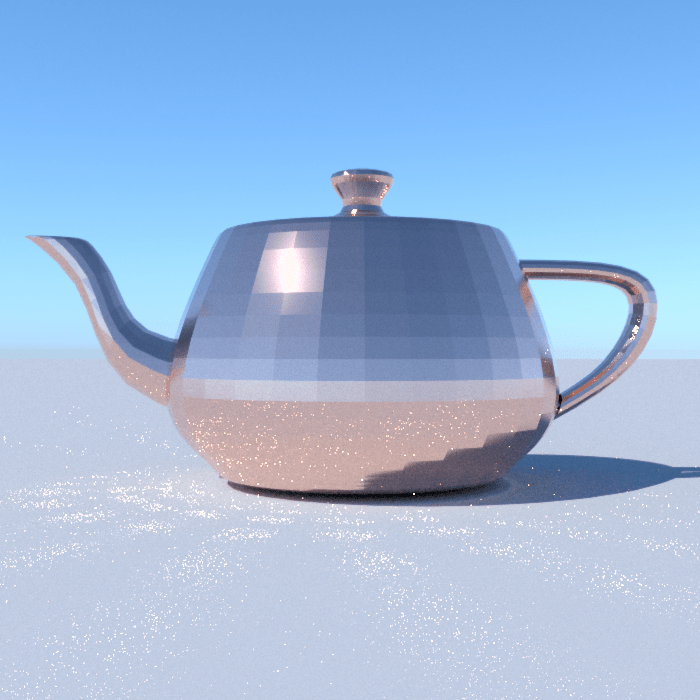
\includegraphics[width=.3\textwidth]{img/4 results/ply/teapotEmbree.png}\label{fig:mesh_teapot}}
	\hfill
	\subfloat[Stanford Bunny]{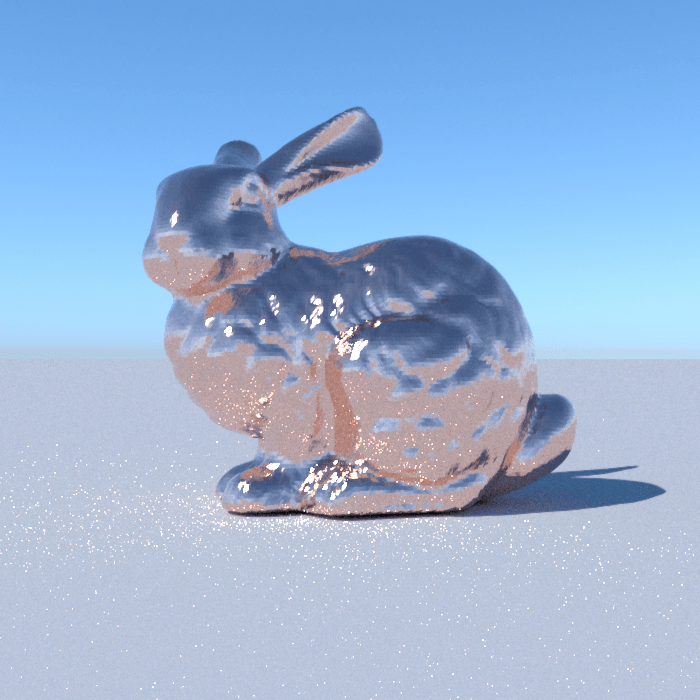
\includegraphics[width=.3\textwidth]{img/4 results/ply/bunnyEmbree.png}\label{fig:mesh_bunny}}
	\hfill
	\subfloat[Michelangel's David]{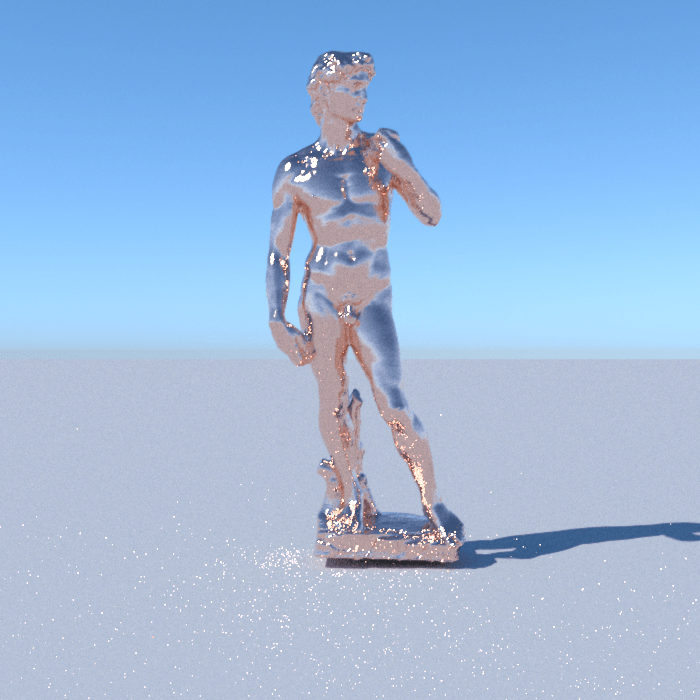
\includegraphics[width=.3\textwidth]{img/4 results/ply/michelangeloEmbree.png}\label{fig:mesh_mike}}
	\\
	\subfloat[Happy Buddha]{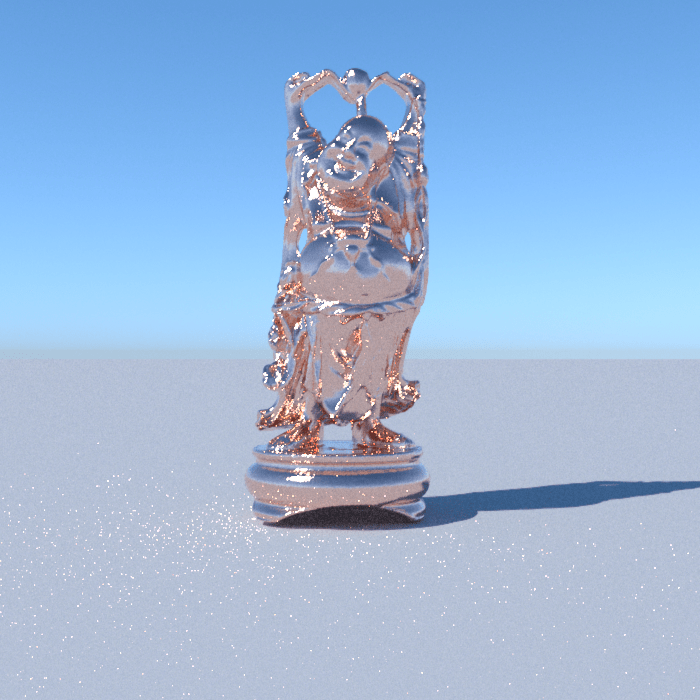
\includegraphics[width=.3\textwidth]{img/4 results/ply/bhuddaEmbree.png}\label{fig:mesh_buddha}}
	\hfill
	\subfloat[Asian Dragon]{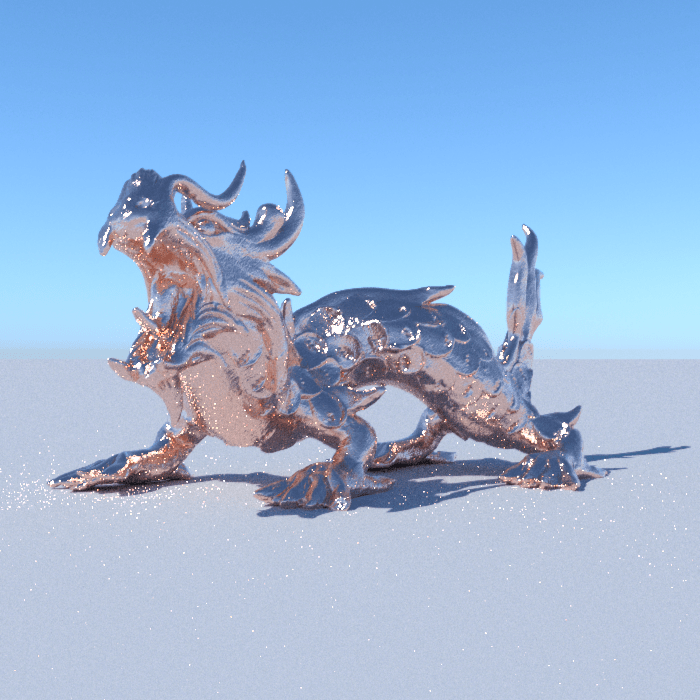
\includegraphics[width=.3\textwidth]{img/4 results/ply/dragonEmbree.png}\label{fig:mesh_dragon}}
	\hfill
	\subfloat[Lucy]{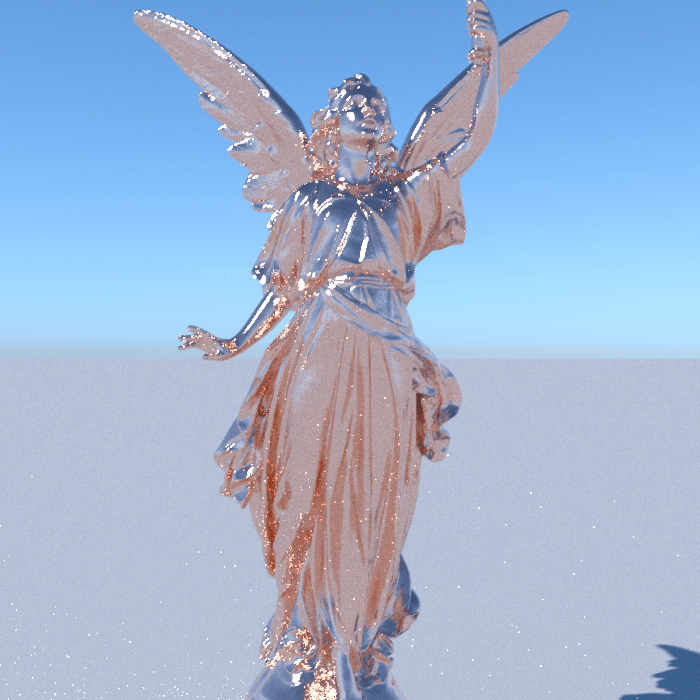
\includegraphics[width=.3\textwidth]{img/4 results/ply/lucyEmbree.png}\label{fig:mesh_lucy}}
	
	\caption{Scenes for triangle meshes}
	\label{fig:mesh_scenes}
\end{figure}


\begin{table}
	\centering
	{\footnotesize\sf
		\begin{tabular}{lrrrrr}
			\toprule
			Scene  & \thead{Native ART \\ Preparation} & \thead{Embree \\ Preparation}  & \thead{Native ART \\ Ray Tracing} & \thead{Embree \\ Ray Tracing} &  \thead{Ray Tracing \\ Speedup}\\ 
			\midrule
			Figure \ref{fig:mesh_teapot} & 0.29 sec & 0.04 sec & 353.83 sec & 304.26 sec &  \textbf{14.01 \%} \\
			Figure \ref{fig:mesh_bunny}  & 4.28 sec & 0.25 sec & 379.02 sec & 305.00 sec &  \textbf{19.53 \%} \\
			Figure \ref{fig:mesh_mike} & 18.40 sec & 1.85 sec &  302.52 sec & 254.03 sec &  \textbf{16.03 \%}  \\
			\addlinespace % a nice non-intrusive separator of data groups (or final table sums)
			Figure \ref{fig:mesh_buddha}  & 57.28 sec & 6.48 sec & 351.92 sec & 276.00 sec &  \textbf{ 21.57 \%} \\
			Figure \ref{fig:mesh_dragon} & (no data)  & 64.43 sec & (no data) & 304.29 sec & (no data)  \\
			Figure \ref{fig:mesh_lucy}  & (no data) & 302.19 sec & (no data) & 327.59 sec & (no data)  \\
			\bottomrule
	\end{tabular}}
	\caption{Comparison between the performances of Native ART and ART with Embree support regarding the rendering of triangle meshes.}
	\label{tab:mesh}
\end{table}

The results in Table \ref{tab:mesh} show a general increase in the performance of ART when supported by Embree. Another advantage of our implementation is the drastic speedup when building the acceleration structure before rendering.

However, we could not render the Asian Dragon and Lucy meshes with Native ART on our local machine. This is because these meshes are large, and so is ART's internal KD tree for grouping the individual triangles into spaces bound by split planes. For triangle meshes composed of a number of triangles higher than a certain threshold, the required memory needed for the construction of the mesh KD tree exceeds the available system memory, which, in our case, results in a termination of the program by the Linux kernel.

At this point, we would like to emphasize that our implementation allows for the rendering of much more complicated scenes than Native ART on the same hardware.